\documentclass[a4paper,12pt]{article}

\usepackage{préambule}

\addtolength{\oddsidemargin}{-0.5cm}
\addtolength{\evensidemargin}{-0.5cm}
\addtolength{\textwidth}{1cm}

\makeatletter
\renewcommand{\maketitle}{%
{\tiny colle dans ton cahier d'exercices}

	\begin{center}
		\LARGE
		\uline{\@title}
		\vspace{1em}
	\end{center}
}
\makeatother

\title{Exercices symétrie centrale}
\date{}
\author{}

\begin{document}

\maketitle

\begin{attention}[frametitle={⚠ Attention ⚠}]
	\center
	Dessine au \textbf{crayon à papier} !
\end{attention}

\noindent
{\large \textbf{En suivant les étapes vues en cours}}, \\
fait le symétrique des figures suivantes par rapport au point $O$ : \\

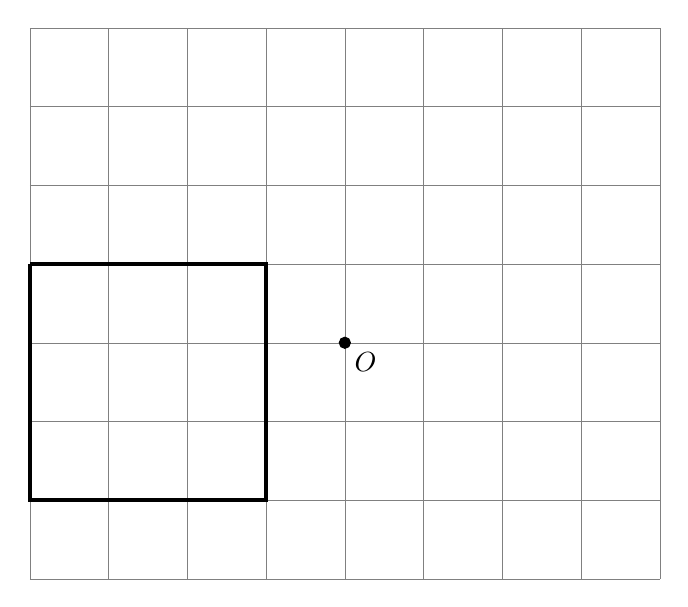
\begin{tikzpicture}
	\draw[step=1,gray,ultra thin] (0,0) grid (8,7);
	\filldraw[black] (4,3) node[anchor=north west] {$O$} circle (2pt);

	\draw[black,ultra thick] (0,4) -- ++(0,-3) -- ++(3,0) -- ++(0,3) -- ++(-3,0);
\end{tikzpicture} \hspace{1em}
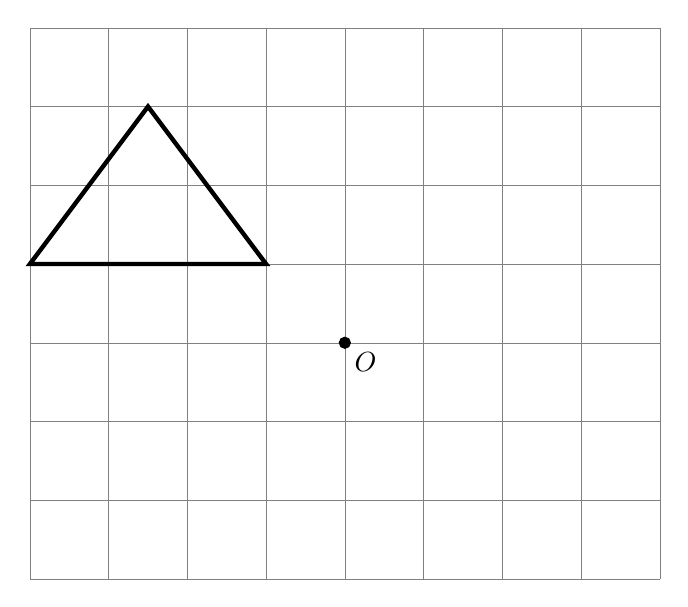
\begin{tikzpicture}
	\draw[step=1,gray,ultra thin] (0,0) grid (8,7);
	\filldraw[black] (4,3) node[anchor=north west] {$O$} circle (2pt);

	\draw[black,ultra thick] (3,4) -- ++(-1.5,2) -- ++(-1.5,-2) -- cycle;
\end{tikzpicture} \vspace{1em}

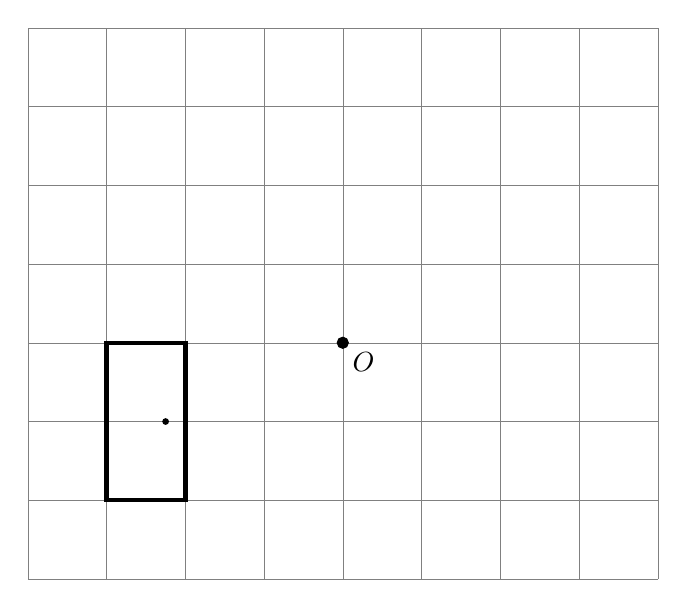
\begin{tikzpicture}
	\draw[step=1,gray,ultra thin] (0,0) grid (8,7);
	\filldraw[black] (4,3) node[anchor=north west] {$O$} circle (2pt);

	\draw[black,ultra thick] (1,1) -- ++(0,2) -- ++(1,0) -- ++(0,-2) -- cycle;
	\filldraw[black] (1.75,2) circle (1pt);
\end{tikzpicture} \hspace{1em}
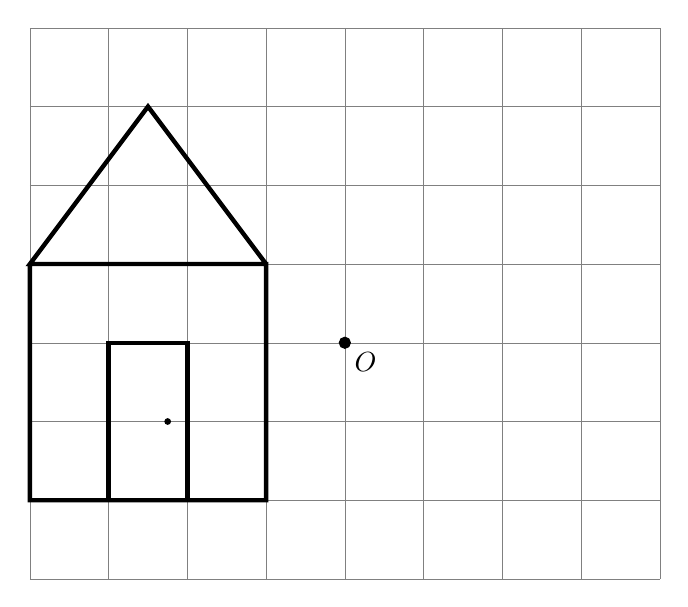
\begin{tikzpicture}
	\draw[step=1,gray,ultra thin] (0,0) grid (8,7);
	\filldraw[black] (4,3) node[anchor=north west] {$O$} circle (2pt);

	\draw[black,ultra thick] (0,4) -- ++(0,-3) -- ++(3,0) -- ++(0,3) -- ++(-3,0) -- ++(1.5,2) -- ++(1.5,-2);
	\draw[black,ultra thick] (1,1) -- ++(0,2) -- ++(1,0) -- ++(0,-2);
	\filldraw[black] (1.75,2) circle (1pt);
\end{tikzpicture}

\end{document}